\appendix
\chapter{Appendix}
\captionsetup{list=no}
\begin{table}[h!]
    \centering
    \begin{tabular}{|c c | c c | c c|} 
        \multicolumn{6}{c}{univariate mmd scores}\\
        \hline
        batch & mmd score & batch & mmd score  & batch & mmd score \\
        \hline\hline
        lsm 01 & 0.001095 &
        lsm 02 & 0.001189 &
        lsm 03 & 0.000248 \\
        lsm 04 & 0.004695 &
        lsm 05 & 0.000790 &
        lsm 06 & 0.022553 \\
        lsm 07 & 0.006913 &
        lsm 08 & \textbf{\textcolor{blue}{0.000203}} &
        lsm 09 & 0.003571 \\
        lsm 10 & 0.001193 &
        lsm 11 & 0.000987 &
        lsm 12 & 0.002153 \\
        lsm 13 & 0.001272 &
        lsm 14 & 0.000353 &
        lsm 15 & 0.000683 \\
        lsm 16 & 0.000852 &
        lsm 17 & 0.001853 &
        lsm 18 & 0.000379 \\
        lsm 19 & 0.004669 &
        lsm 20 & 0.001623 &
        lsm 21 & 0.001134 \\
        lsm 22 & 0.003864 &
        lsm 23 & 0.001535 &
        lsm 24 & 0.001667 \\
        lsm 25 & 0.004149 &
        lsm 26 & 0.010215 &
        lsm 27 & 0.007429 \\
        lsm 28 & 0.000372 &
        lsm 29 & 0.006910 &
        lsm 30 & 0.002412 \\
        lsm 31 & 0.003552 &
        lsm 32 & 0.000283 &
        lsm 33 & 0.006011 \\
        lsm 34 & 0.005022 &
        lsm 35 & 0.000650 &
        lsm 36 & 0.001387 \\
        lsm 37 & 0.005250 &
        lsm 38 & 0.004809 &
        lsm 39 & 0.006311 \\
        lsm 40 & 0.001373 &
        lsm 41 & 0.000411 &
        lsm 42 & 0.000560 \\
        lsm 43 & \textbf{\textcolor{red}{0.030736}} &
        lsm 44 & 0.000643 &
        lsm 45 & 0.001401 \\
        lsm 46 & 0.004326 &
        lsm 47 & 0.002762 &
        lsm 48 & 0.000899 \\
        lsm 49 & 0.002654 &
        lsm 50 & 0.002061 &
        lsm 51 & 0.001648 \\
        lsm 52 & 0.006343 &
        lsm 53 & 0.002718 &
        lsm 54 & 0.003370 \\
        \hline
        \multicolumn{6}{c}{mean: 0.003569}
    \end{tabular}

    \begin{tabular}{|c c |c c| c c|}
        \multicolumn{6}{c}{multivariate mmd scores}\\
        \hline
        batch & mmd score & batch & mmd score & batch & mmd score\\
        \hline\hline
        lsm 01 & 0.004302 &
        lsm 02 & 0.001880 &
        lsm 03 & 0.001095 \\
        lsm 04 & 0.002974 &
        lsm 05 & 0.005337 &
        lsm 06 & 0.006210 \\
        lsm 07 & 0.004319 &
        lsm 08 & 0.005429 &
        lsm 09 & 0.007599 \\
        lsm 10 & 0.001365 &
        lsm 11 & 0.002206 &
        lsm 12 & 0.004846 \\
        lsm 13 & 0.002317 &
        lsm 14 & 0.002696 &
        lsm 15 & 0.001315 \\
        lsm 16 & 0.000821 &
        lsm 17 & 0.012402 &
        lsm 18 & 0.008775 \\
        lsm 19 & 0.014695 &
        lsm 20 & 0.002632 &
        lsm 21 & 0.003236 \\
        lsm 22 & 0.001471 &
        lsm 23 & 0.005080 &
        lsm 24 & 0.006379 \\
        lsm 25 & 0.001095 &
        lsm 26 & 0.003414 &
        lsm 27 & 0.011945 \\
        lsm 28 & 0.002359 &
        lsm 29 & 0.003644 &
        lsm 30 & 0.007566 \\
        lsm 31 & 0.007163 &
        lsm 32 & \textbf{\textcolor{red}{0.036864}}&
        lsm 33 & 0.007520 \\
        lsm 34 & 0.006216 &
        lsm 35 & 0.008992 &
        lsm 36 & 0.004288 \\
        lsm 37 & 0.002008 &
        lsm 38 & 0.011144 &
        lsm 39 & 0.004037 \\
        lsm 40 & 0.001489 &
        lsm 41 & 0.002060 &
        lsm 42 & 0.013073 \\
        lsm 43 & 0.009164 &
        lsm 44 & 0.001884 &
        lsm 45 & 0.001099 \\
        lsm 46 & 0.002816 &
        lsm 47 & 0.011187 &
        lsm 48 & 0.001550 \\
        lsm 49 & 0.001935 &
        lsm 50 & 0.001988 &
        lsm 51 & 0.006244 \\
        lsm 52 & 0.005689 &
        lsm 53 & 0.004562 &
        lsm 54 & \textbf{\textcolor{blue}{0.000449}}\\
        \hline
        \multicolumn{6}{c}{mean: 0.005349}
    \end{tabular}
    \caption{All mmd score results for univariate and multivariate LSM models.}
    \label{table:lsm results}
\end{table}
\begin{figure}
    \centering
    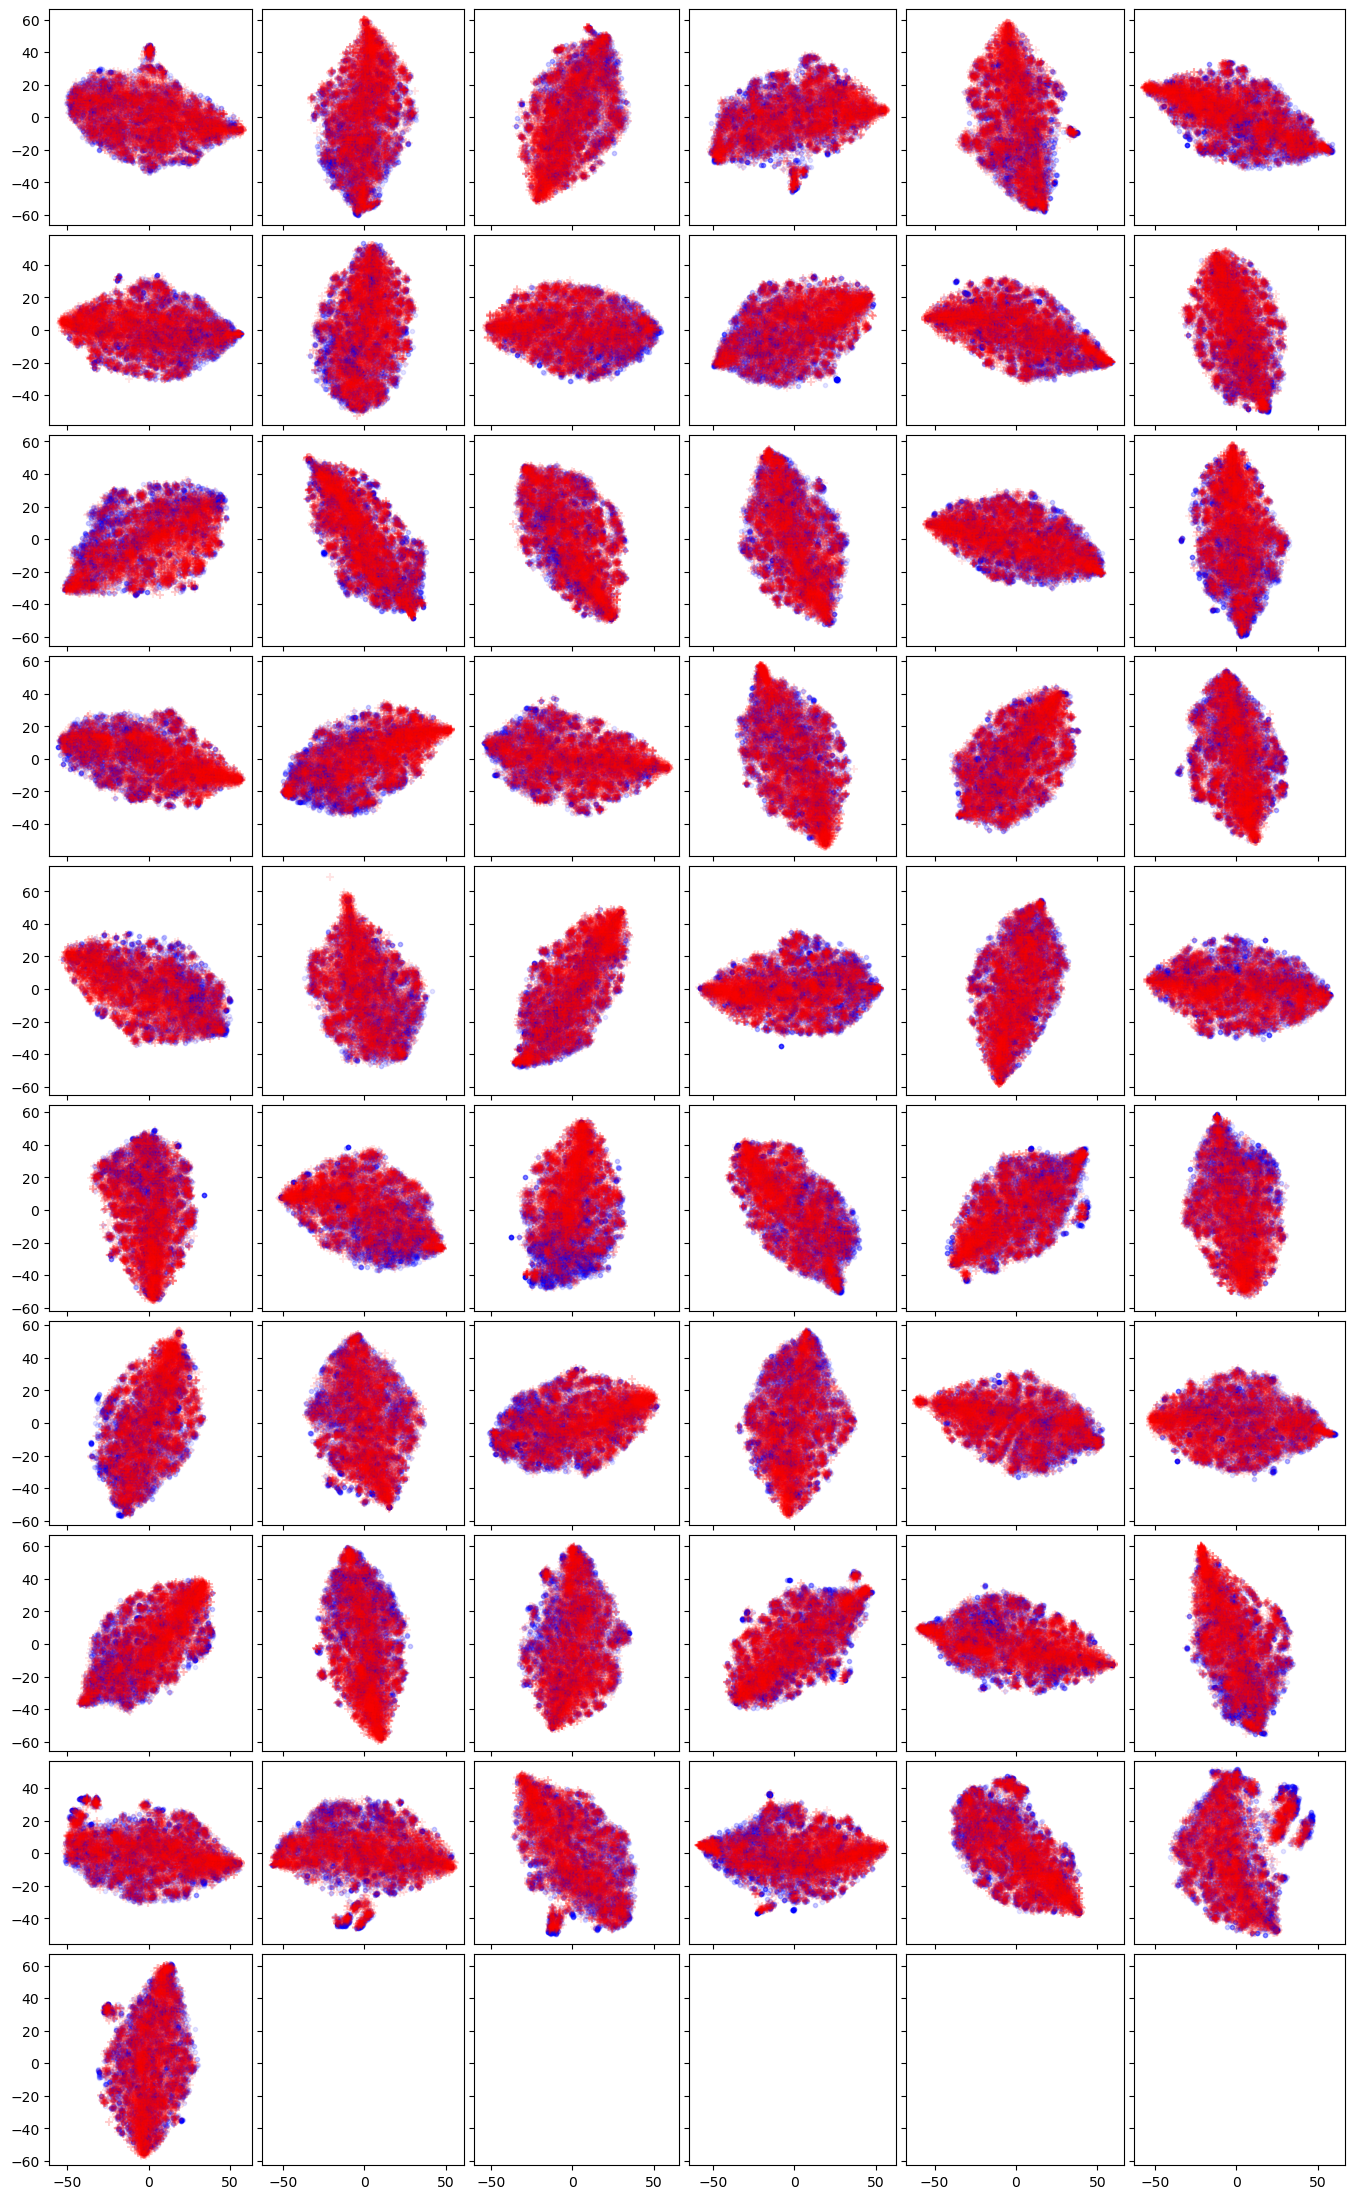
\includegraphics[height=\textheight]{images/tsen_overall_mult.png}
    \caption{TSNE batch results for multivariate experiments.}
    \label{fig:tsne overall mult}
\end{figure}
\begin{figure}
    \centering
    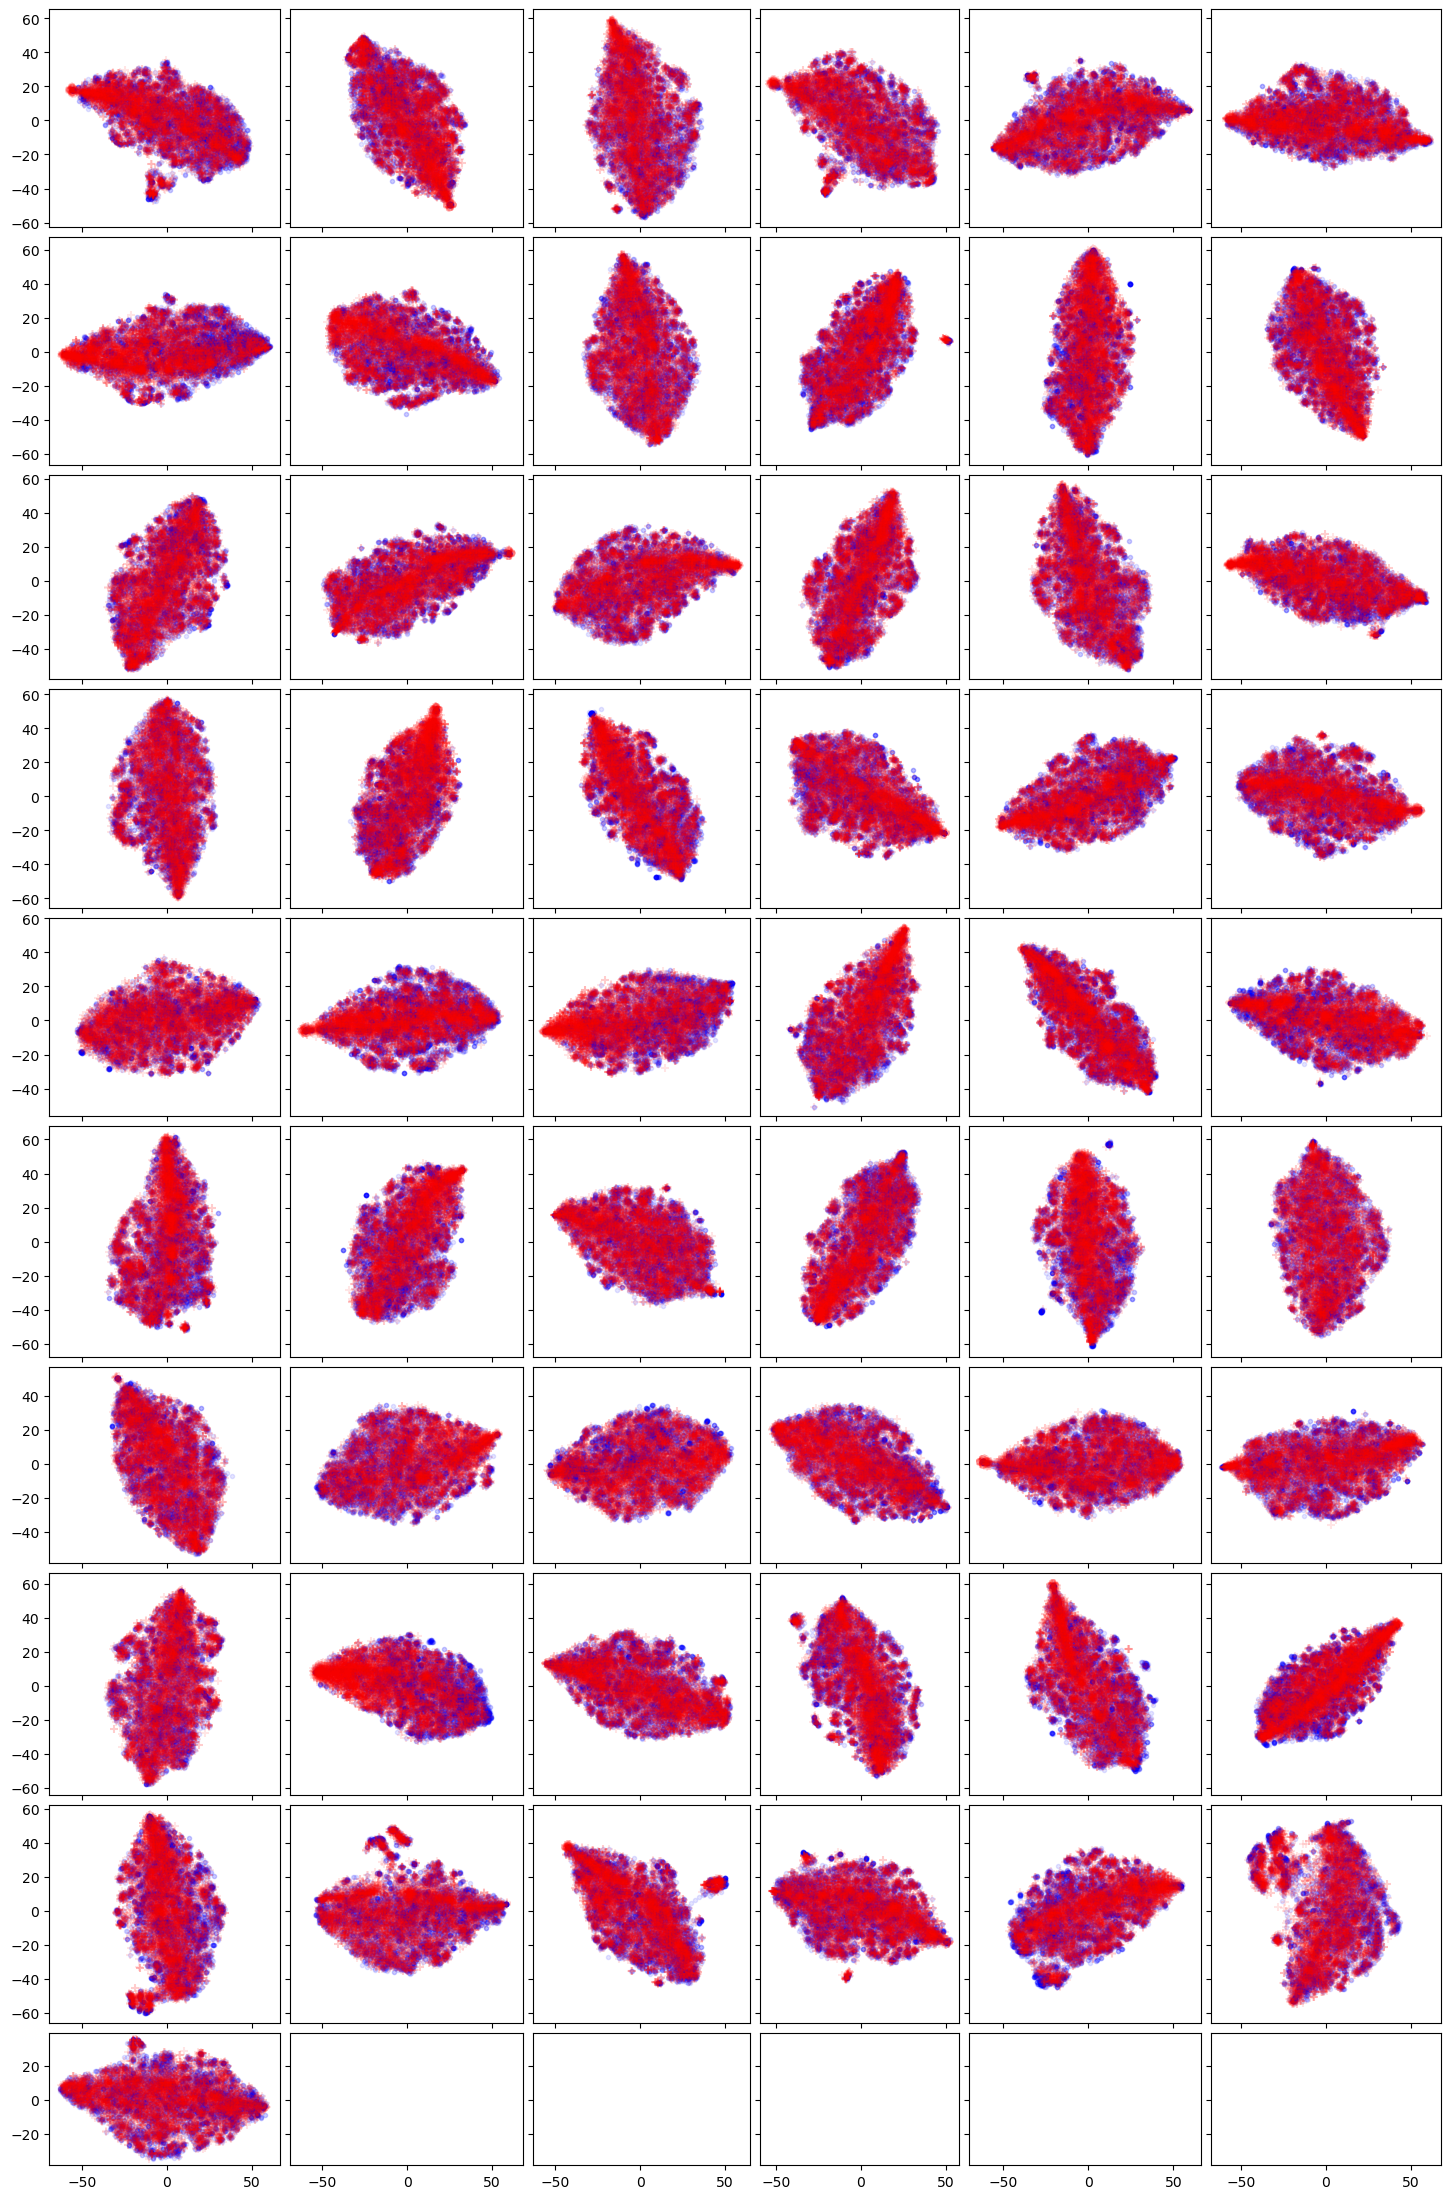
\includegraphics[height=\textheight]{images/tsen_overall_uni.png}
    \caption{TSNE batch results for univariate experiments.}
    \label{fig:tsne overall uni}
\end{figure}
\begin{figure}
    \centering
    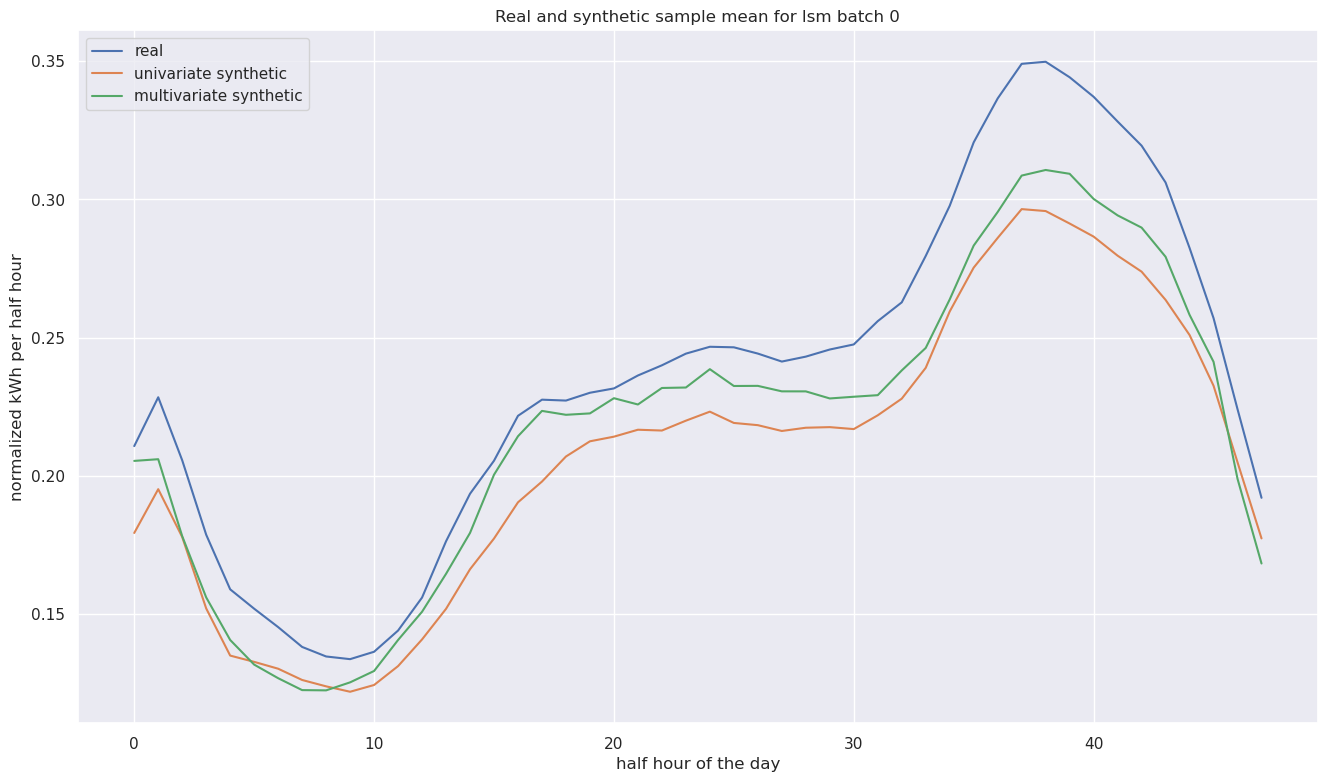
\includegraphics[width=\textwidth]{images/lsm_dm_0.png}
    \caption{Real and generated sample mean for lsm batch 0}
    \label{fig:sample mean 09}
\end{figure}
\begin{figure}
    \centering
    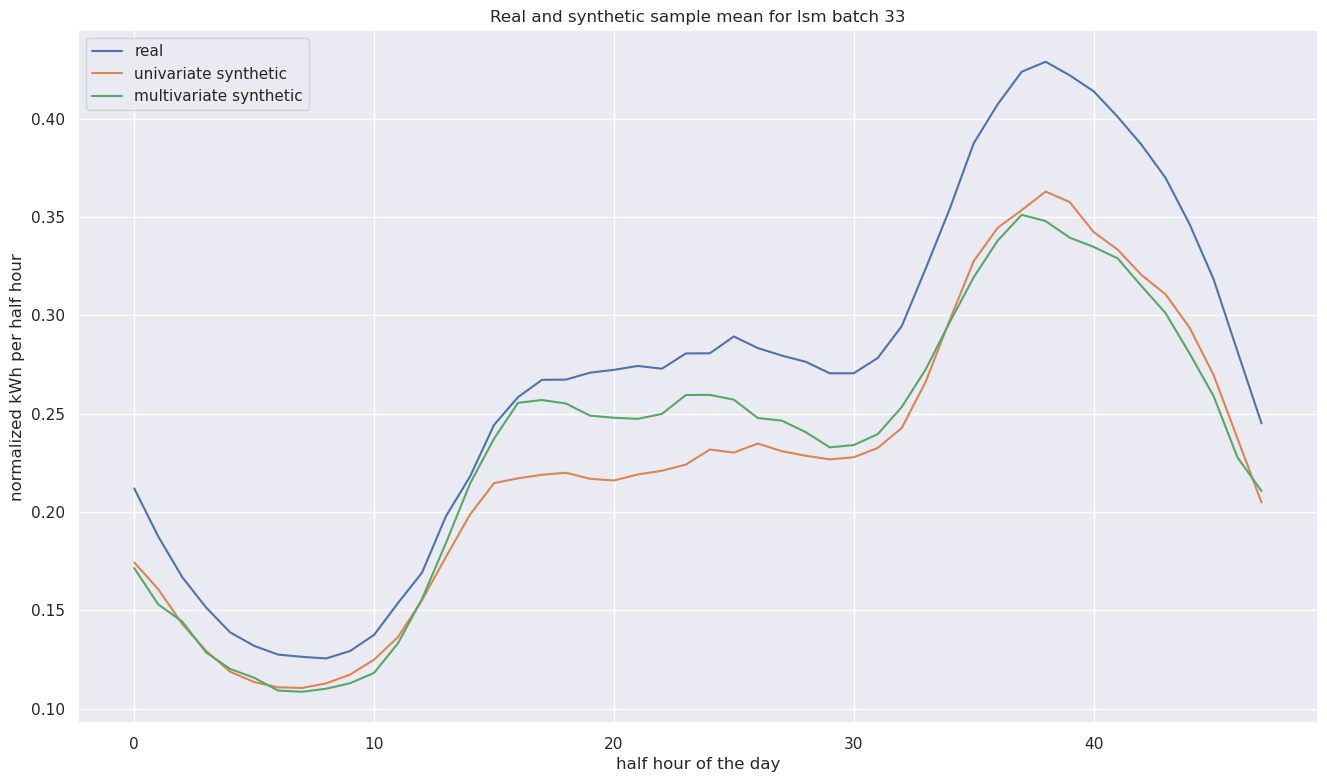
\includegraphics[width=\textwidth]{images/lsm_dm_33.png}
    \caption{Real and generated sample mean for lsm batch 33}
    \label{fig:sample mean 37}
\end{figure}
\begin{figure}
    \centering
    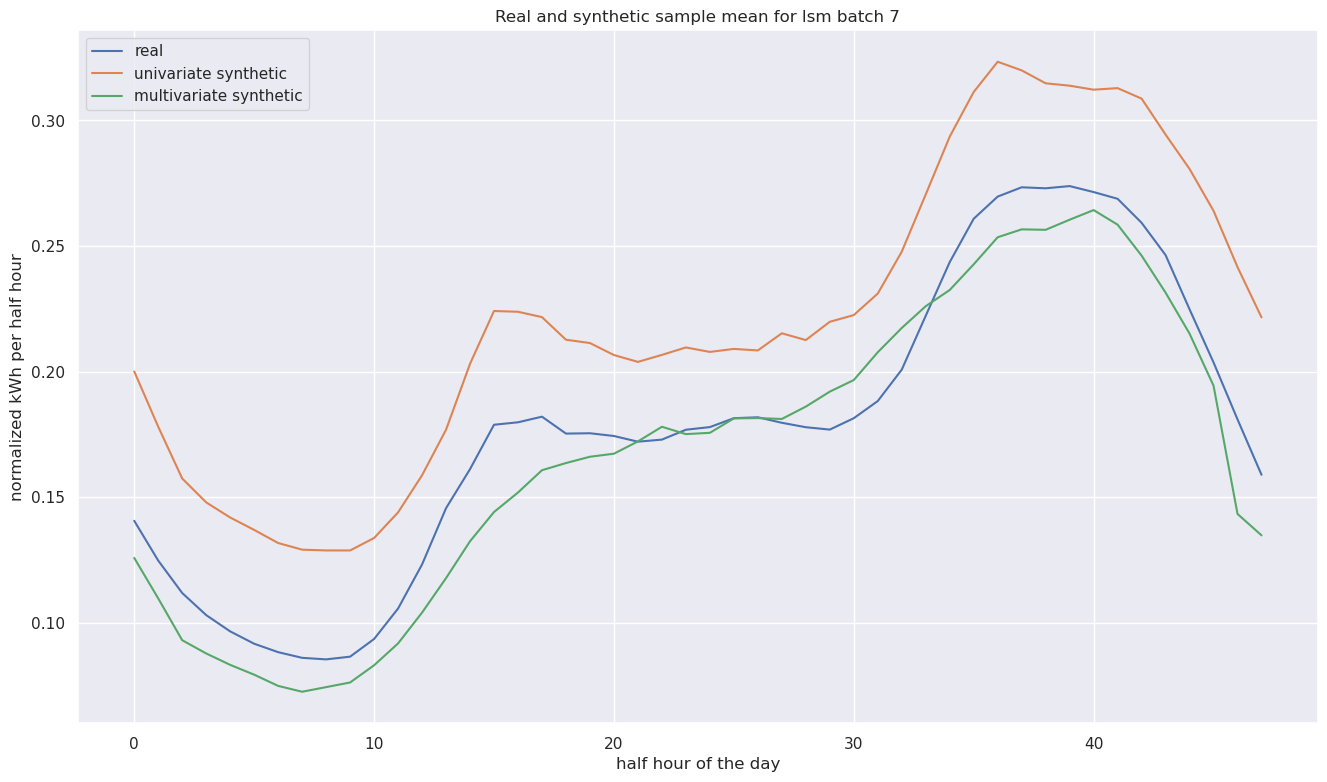
\includegraphics[width=\textwidth]{images/lsm_dm_7.png}
    \caption{Real and generated sample mean for lsm batch 7}
    \label{fig:sample mean 53}
\end{figure}
\begin{figure}
    \centering
    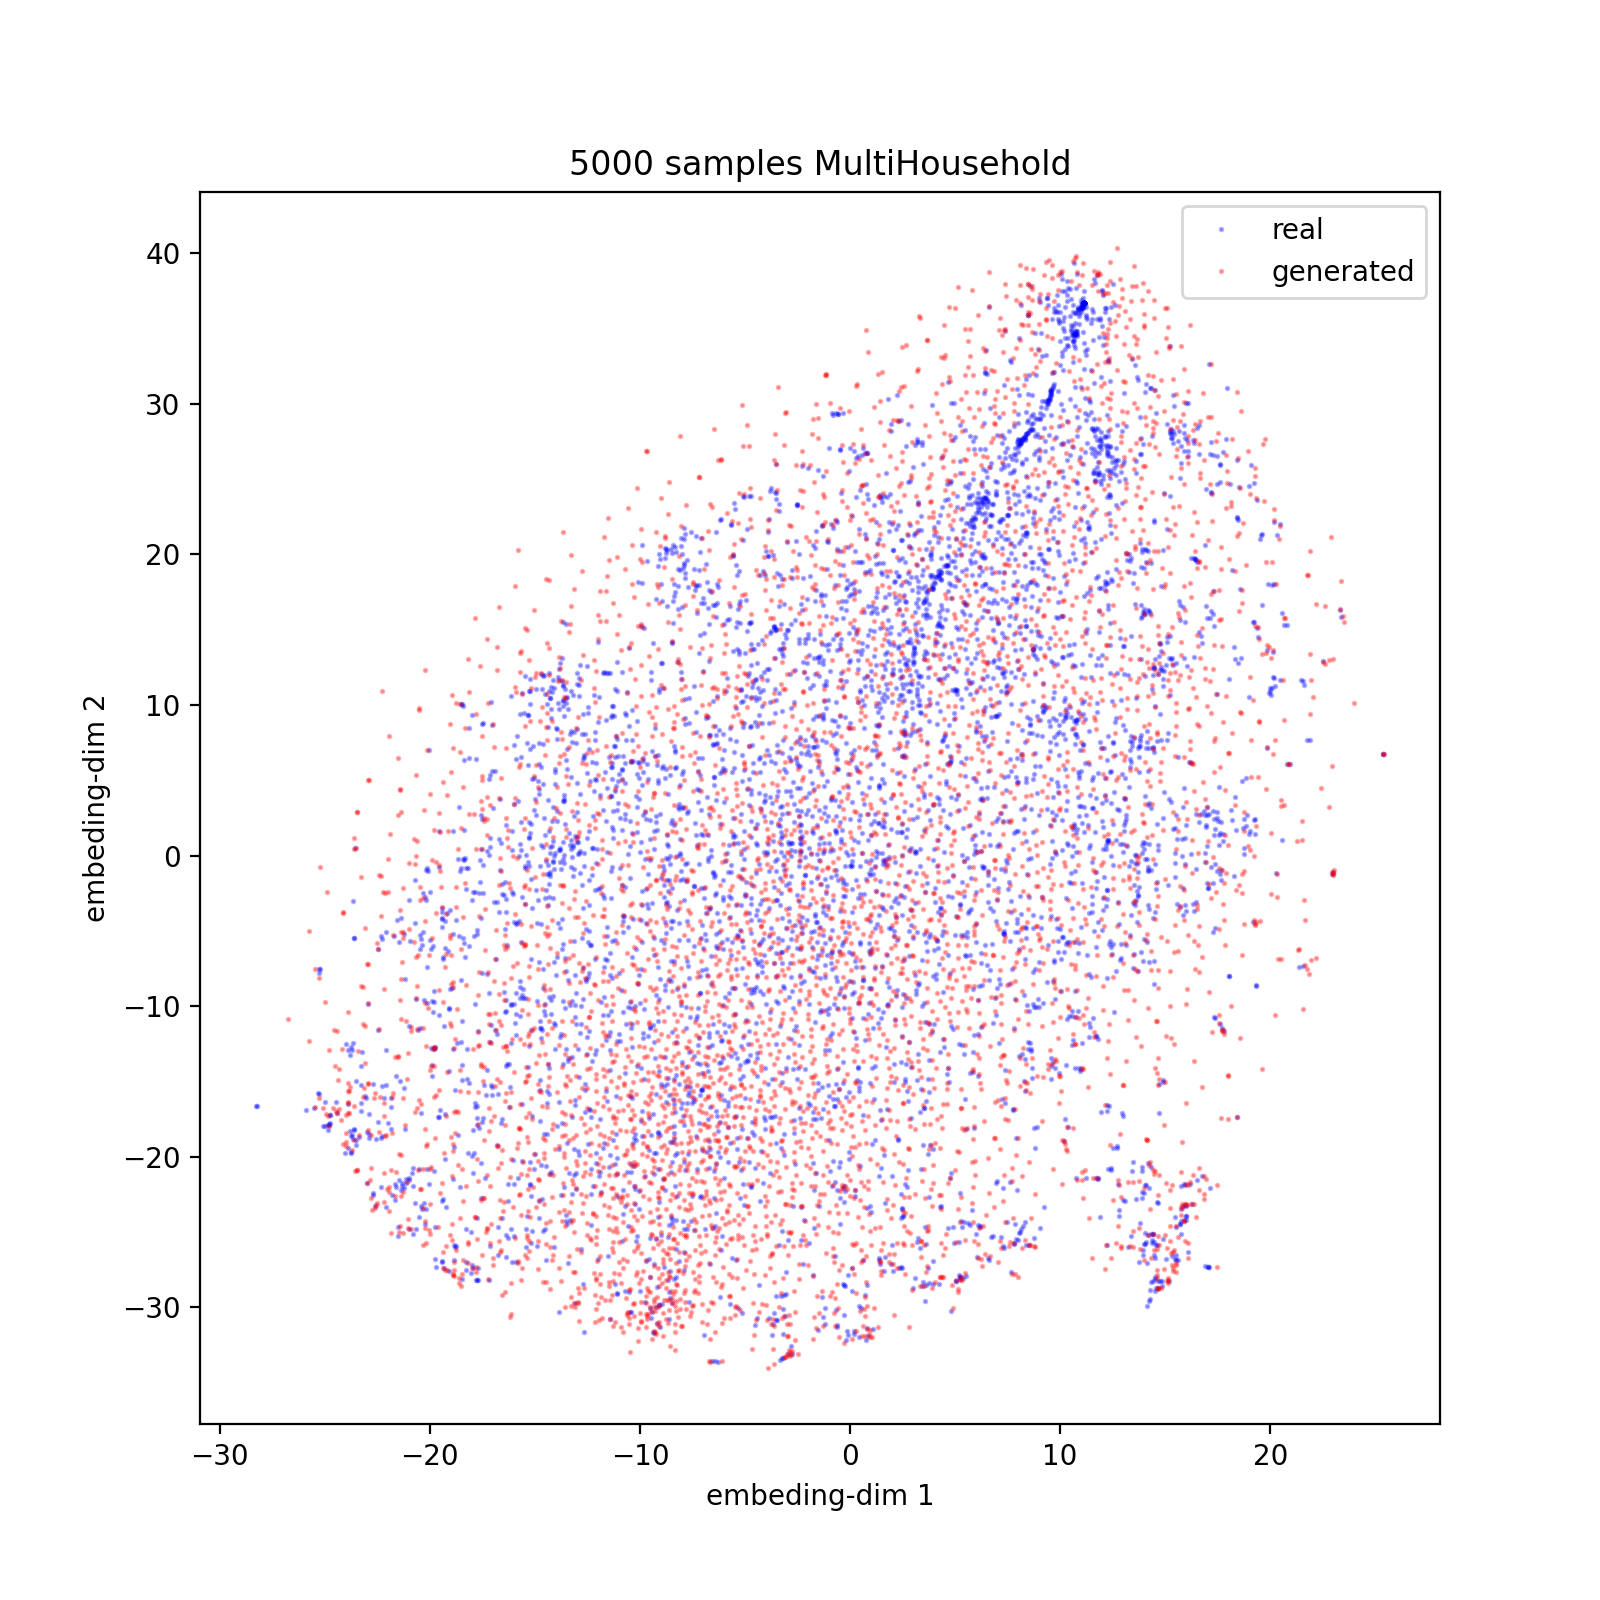
\includegraphics[width=0.85\textwidth]{images/om_uni_tsne.png}
    \caption{Univariate t-SNE samples from openmeter experiments.}
    \label{fig:om tsne uni}
\end{figure}
\begin{figure}
    \centering
    \begin{subfigure}[b]{0.45\textwidth}
        \centering
        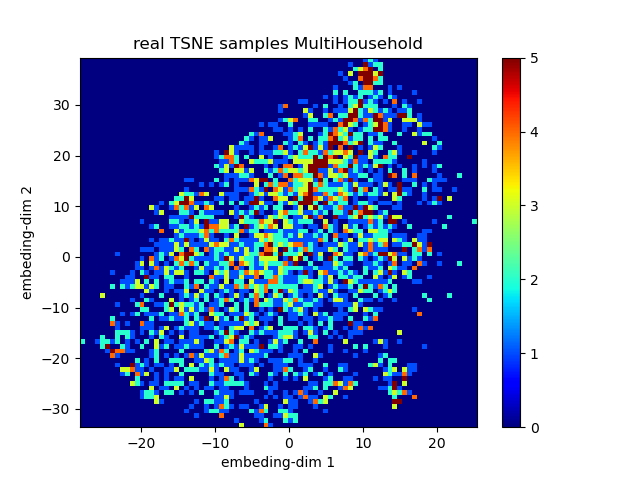
\includegraphics[width=\textwidth]{images/om_uni_real_histo.png}
        \caption{Univariate openmeter t-SNE histogram for real samples.}
        \label{fig:om tsne uni real histo}
    \end{subfigure}
    \begin{subfigure}[b]{0.45\textwidth}
        \centering
        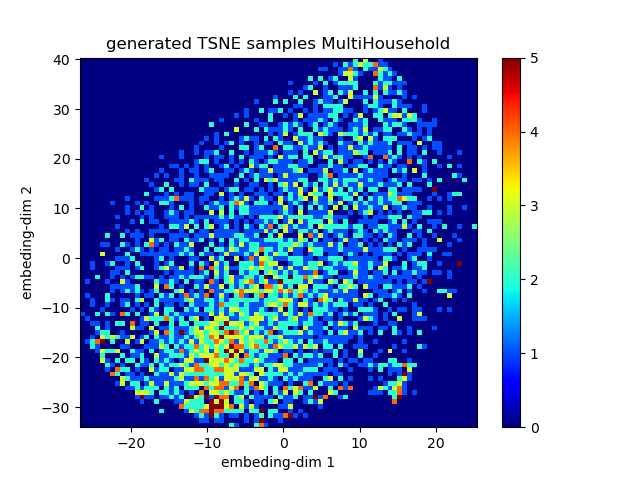
\includegraphics[width=\textwidth]{images/om_uni_fake_histo.png}
        \caption{Univariate openmeter t-SNE histogram for fake samples.}
        \label{fig:om tsne uni fake histo}
    \end{subfigure}
       \caption{Histogram of real and fake t-SNE samples for comparison.}
       \label{fig:om tsne uni histo}
\end{figure}

\begin{figure}
    \centering
    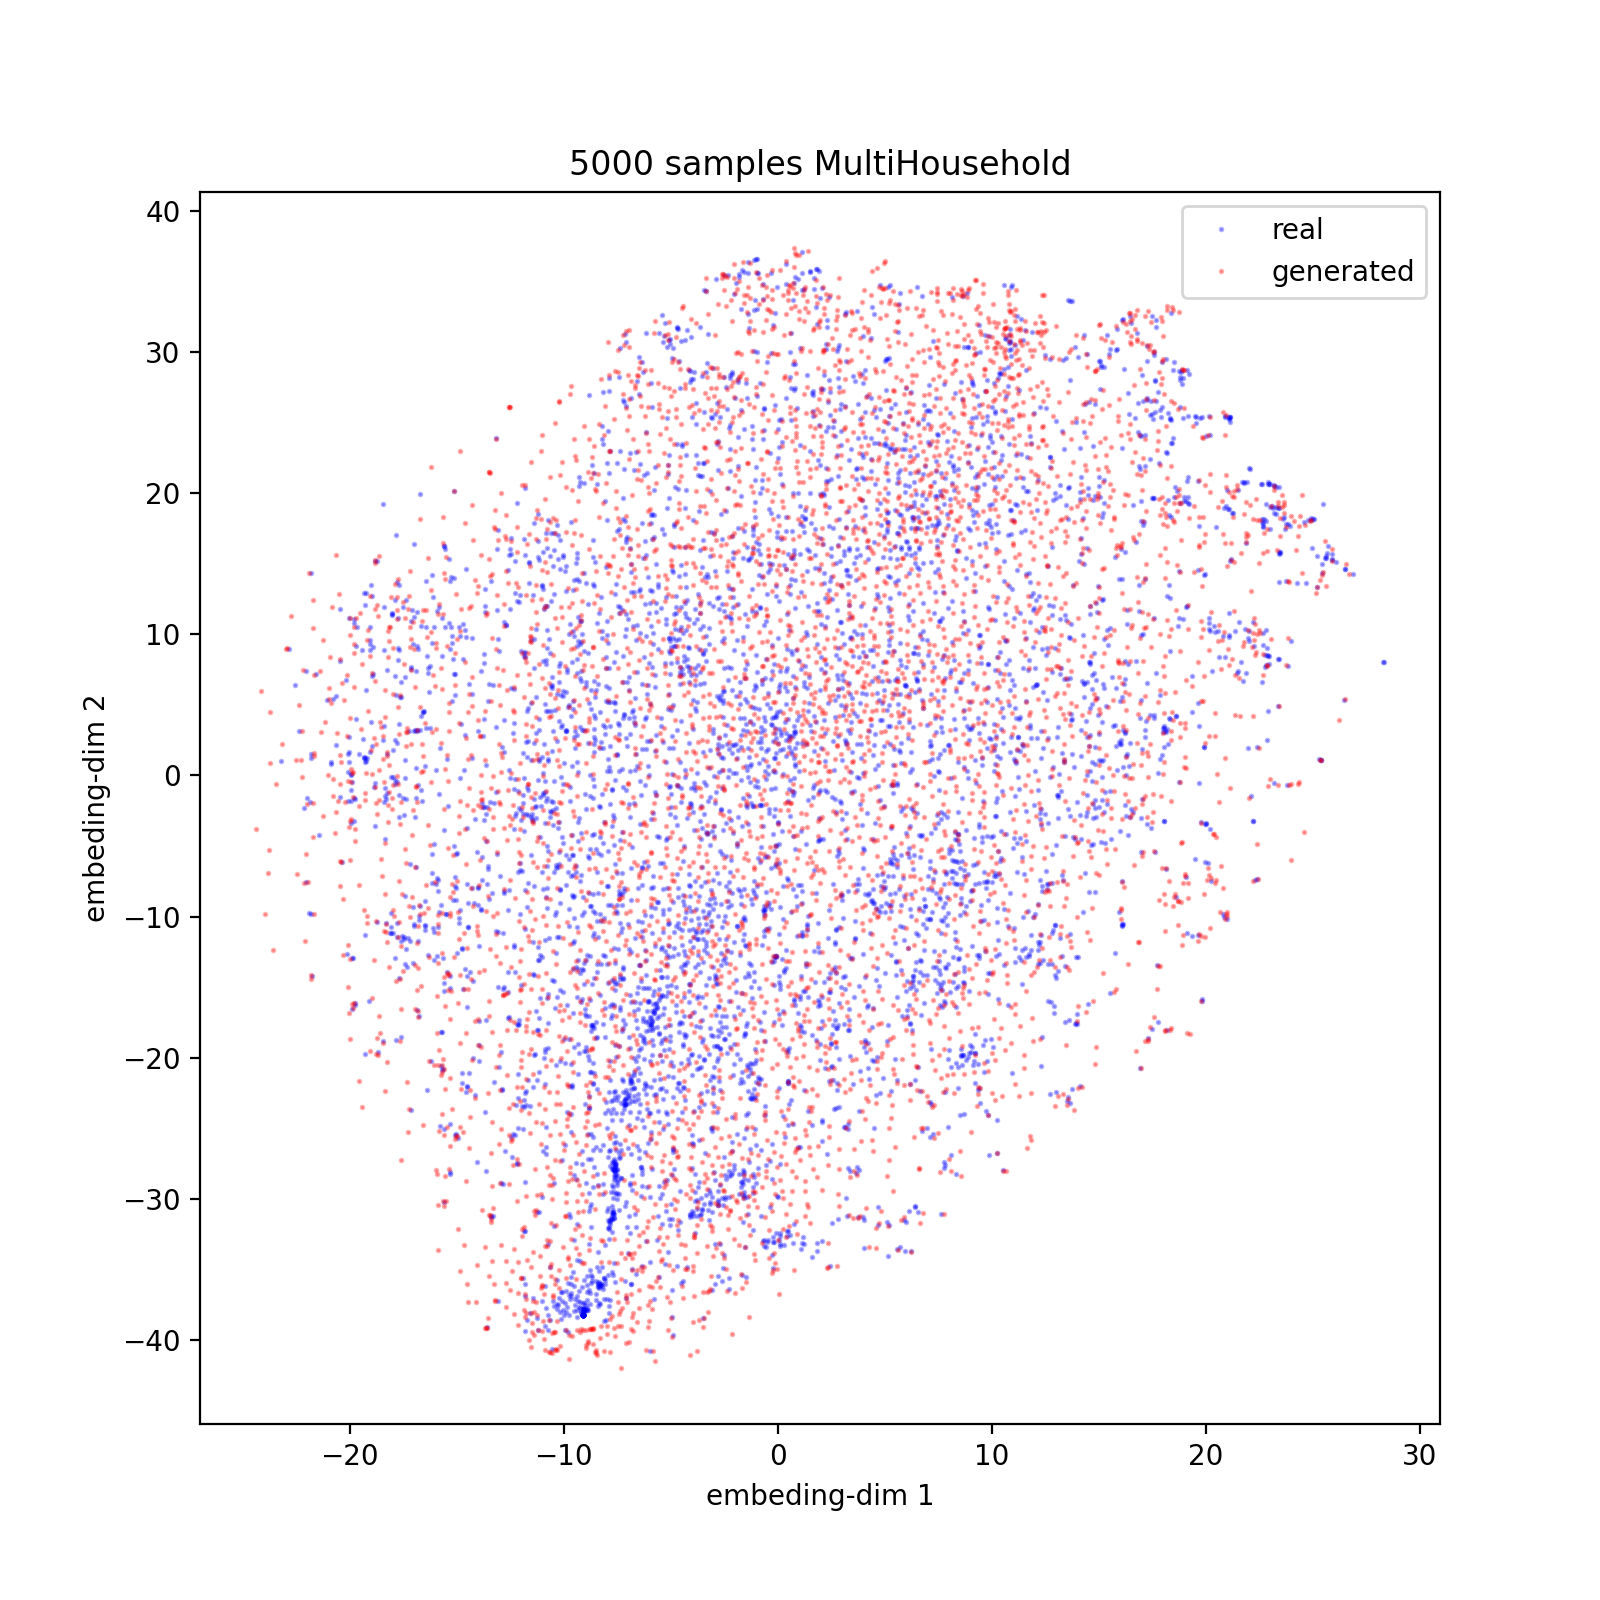
\includegraphics[width=0.85\textwidth]{images/om_multi_tsne.png}
    \caption{Multivariate t-SNE samples from openmeter experiments.}
    \label{fig:om tsne multi}
\end{figure}
\begin{figure}
    \centering
    \begin{subfigure}[b]{0.45\textwidth}
        \centering
        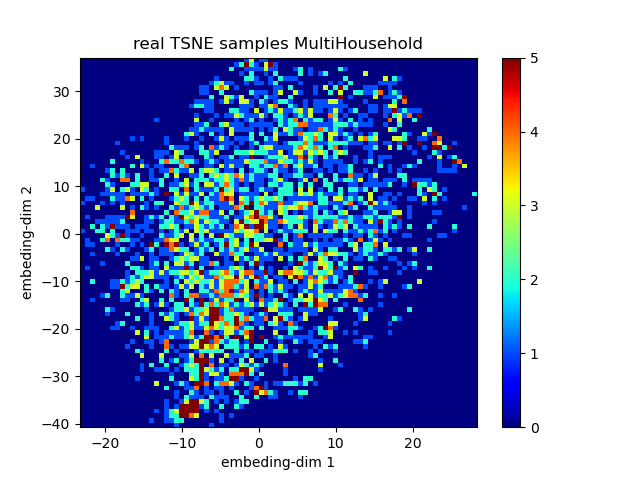
\includegraphics[width=\textwidth]{images/om_multi_real_histo.png}
        \caption{Multivariate openmeter t-SNE histogram for real samples.}
        \label{fig:om tsne multi real histo}
    \end{subfigure}
    \begin{subfigure}[b]{0.45\textwidth}
        \centering
        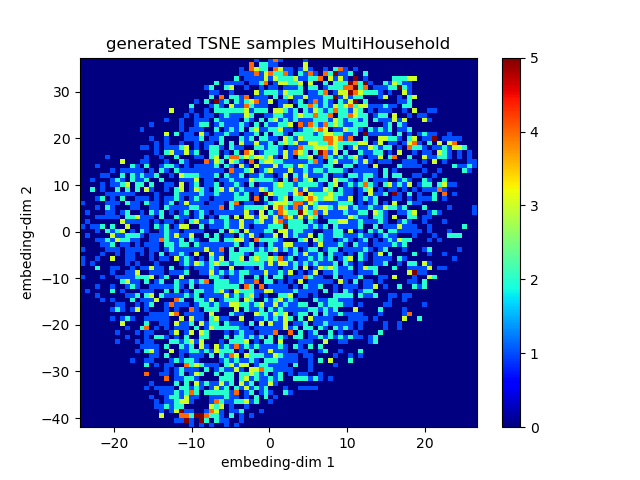
\includegraphics[width=\textwidth]{images/om_multi_fake_histo.png}
        \caption{Multivariate openmeter t-SNE histogram for fake samples.}
        \label{fig:om tsne multi fake histo}
    \end{subfigure}
       \caption{Histogram of real and fake t-SNE samples for comparison.}
       \label{fig:om tsne multi histo}
\end{figure}